% Gemini theme
% https://github.com/anishathalye/gemini
%
% We try to keep this Overleaf template in sync with the canonical source on
% GitHub, but it's recommended that you obtain the template directly from
% GitHub to ensure that you are using the latest version.

\documentclass[final]{beamer}

% ====================
% Packages
% ====================

\usepackage[T1]{fontenc}
\usepackage{lmodern}
% \usepackage[size=custom,width=120,height=72,scale=1.0]{beamerposter}
% \usepackage[size=custom,width=48in,height=36in,scale=1.0]{beamerposter}
% \usepackage[paperheight=36in,paperwidth=48in,showframe]{geometry}
\usepackage[size=custom,width=30in,height=40in,scale=1.0]{beamerposter}

\usetheme{gemini}
\usecolortheme{mit}
\usepackage{graphicx}
\usepackage{booktabs}
\usepackage{tikz}
% \usepackage{pgfplots}
% \pgfplotsset{width=30cm, compat=1.9}
\usepackage{fancyhdr}


\usepackage{pgf}
\usepackage{lmodern}
\usepackage{import}
% \import{figures}{persistence_diagram.pgf}
% ====================
% Lengths
% ====================

% If you have N columns, choose \sepwidth and \colwidth such that
% (N+1)*\sepwidth + N*\colwidth = \paperwidth
\newlength{\sepwidth}
\newlength{\colwidth}
\setlength{\sepwidth}{0.025\paperwidth}
\setlength{\colwidth}{0.4625\paperwidth}

\newcommand{\separatorcolumn}{\begin{column}{\sepwidth}\end{column}}

% ====================
% Title
% ====================

\title{Efficient EHR Foundational Models: A Mixture-of-Experts Approach for Patient Timeline Prediction}

\author{Sudhanva Manjunath Athreya \and Matthias Christenson \and Warren Woodrich Pettine}

\institute{AI Summit 2025}


% ====================
% Footer (optional)
% ====================

% \footercontent{
%   \href{https://www.example.com}{https://www.example.com} \hfill
%   ABC Conference 2025, New York --- XYZ-1234 \hfill
%   \href{mailto:alyssa.p.hacker@example.com}{alyssa.p.hacker@example.com}}
% % (can be left out to remove footer)

% ====================
% Logo (optional)
% ====================

% use this to include logos on the left and/or right side of the header:
% \logoright{\includegraphics[height=7cm]{logo1.pdf}}
% \logoleft{\includegraphics[height=7cm]{logo2.pdf}}

% ====================
% Body
% ====================


% \titlegraphic{
\includegraphics[width=\paperwidth]{header.png}}

\begin{document}

\begin{frame}[t]
% \maketitle
\begin{columns}[t]
\separatorcolumn

\begin{column}{\colwidth}

  \begin{alertblock} {Problem Statement}
    Hospitals face challenges in predicting critical patient outcomes like mortality and ICU stays. 
    Traditional rule-based systems, unable to capture complex EHR patterns, are falling short. 
    While Generative AI offers promise for predicting patient timelines from large EHR datasets, training these models is computationally expensive due to the high dimensionality and sparsity of EHR data.
    \end{alertblock}

    \begin{block} {Background \& Motivation}
        
        \begin{itemize}
            \item Clinical event prediction improves patient care and resource allocation.
            \item EHR systems cannot capture intricate semantic and temporal pattern in patient data.
            \item Foundational models show potential for predicting patient trajectories.
            \item High dimensionality and sparsity increase training costs.
        \end{itemize}

    \end{block}

    \begin{block}{Data Processing \& Tokenization}

      \begin{figure}
        \centering
        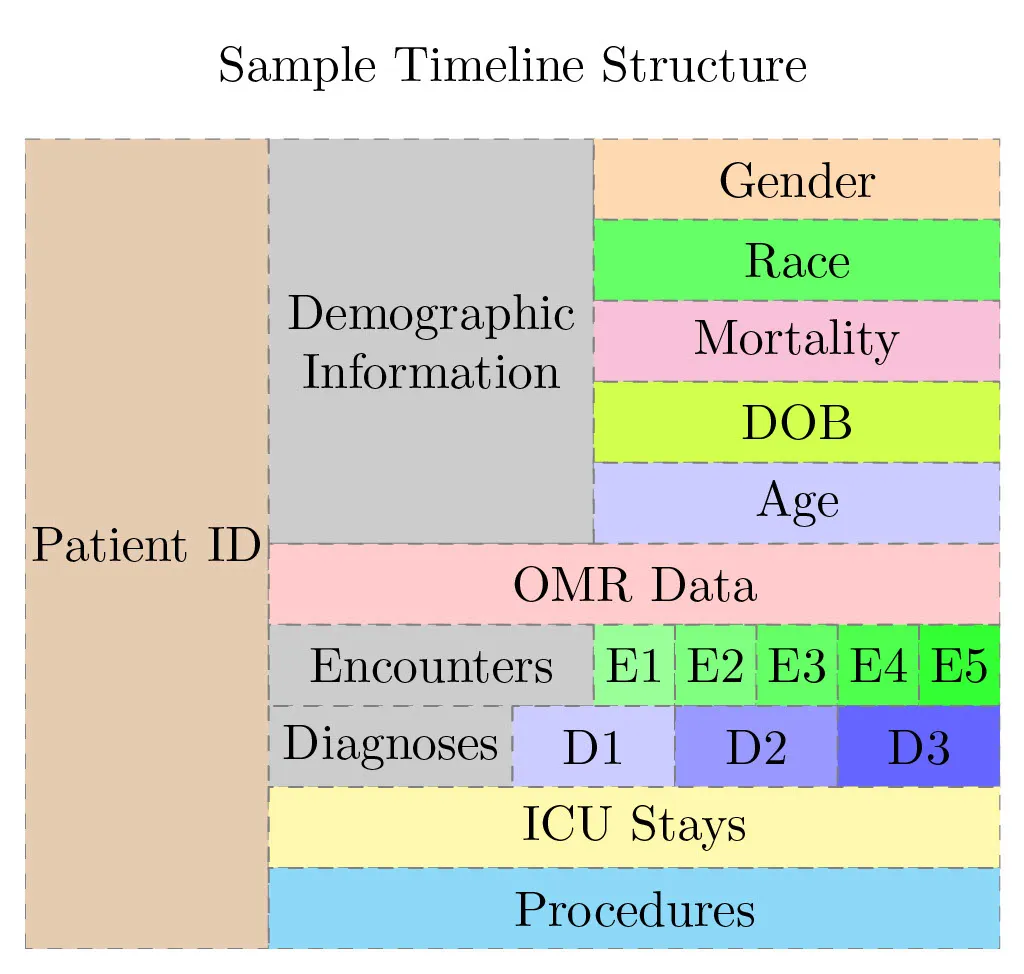
\includegraphics[width=0.6\colwidth]{figures/ehr_timeline.png}
        \caption{\large Patient EHR Timeline Representation}
        \label{fig:ehr_timeline}
      \end{figure}
  
  
      % IMAGE: EHR Data Processing Pipeline
      \begin{figure}
          \centering
          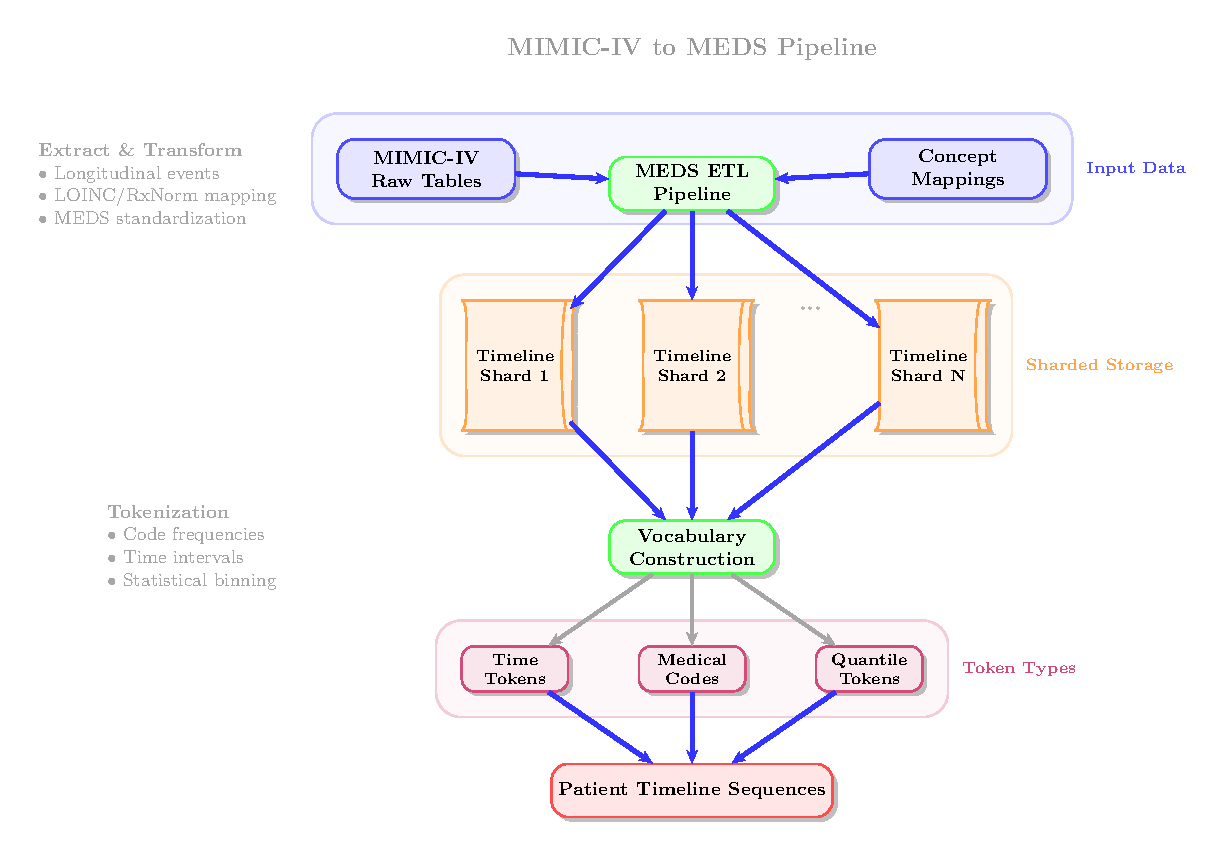
\includegraphics[width=1\linewidth]{figures/ehr_preprocessing_pipeline.pdf}
          \caption{\large EHR Data Processing \& Tokenization Pipeline}
          \label{fig:preprocessing_pipeline}
      \end{figure}
  
    \end{block}    


\end{column}

\separatorcolumn

\begin{column}{\colwidth}


  \begin{block}{Our Approach: Mixture-of-Experts (MoE)}

    % MoE enhances model capacity by employing multiple specialized sub-models (experts) while maintaining computational efficiency through sparse activation.

    % \textbf{Key Components:}
    % \begin{enumerate}
    %     \item \textbf{Multiple Experts:} Linear FFN layers are replaced with multiple experts. 
    %     \item \textbf{Gating Mechanism:} Learned router selects relevant experts using Top-k gating mechanism.
    %     \item \textbf{Sparse Activation:} Only subset of experts activated for an input token.
    %   \end{enumerate}

      \begin{figure}
          \centering
          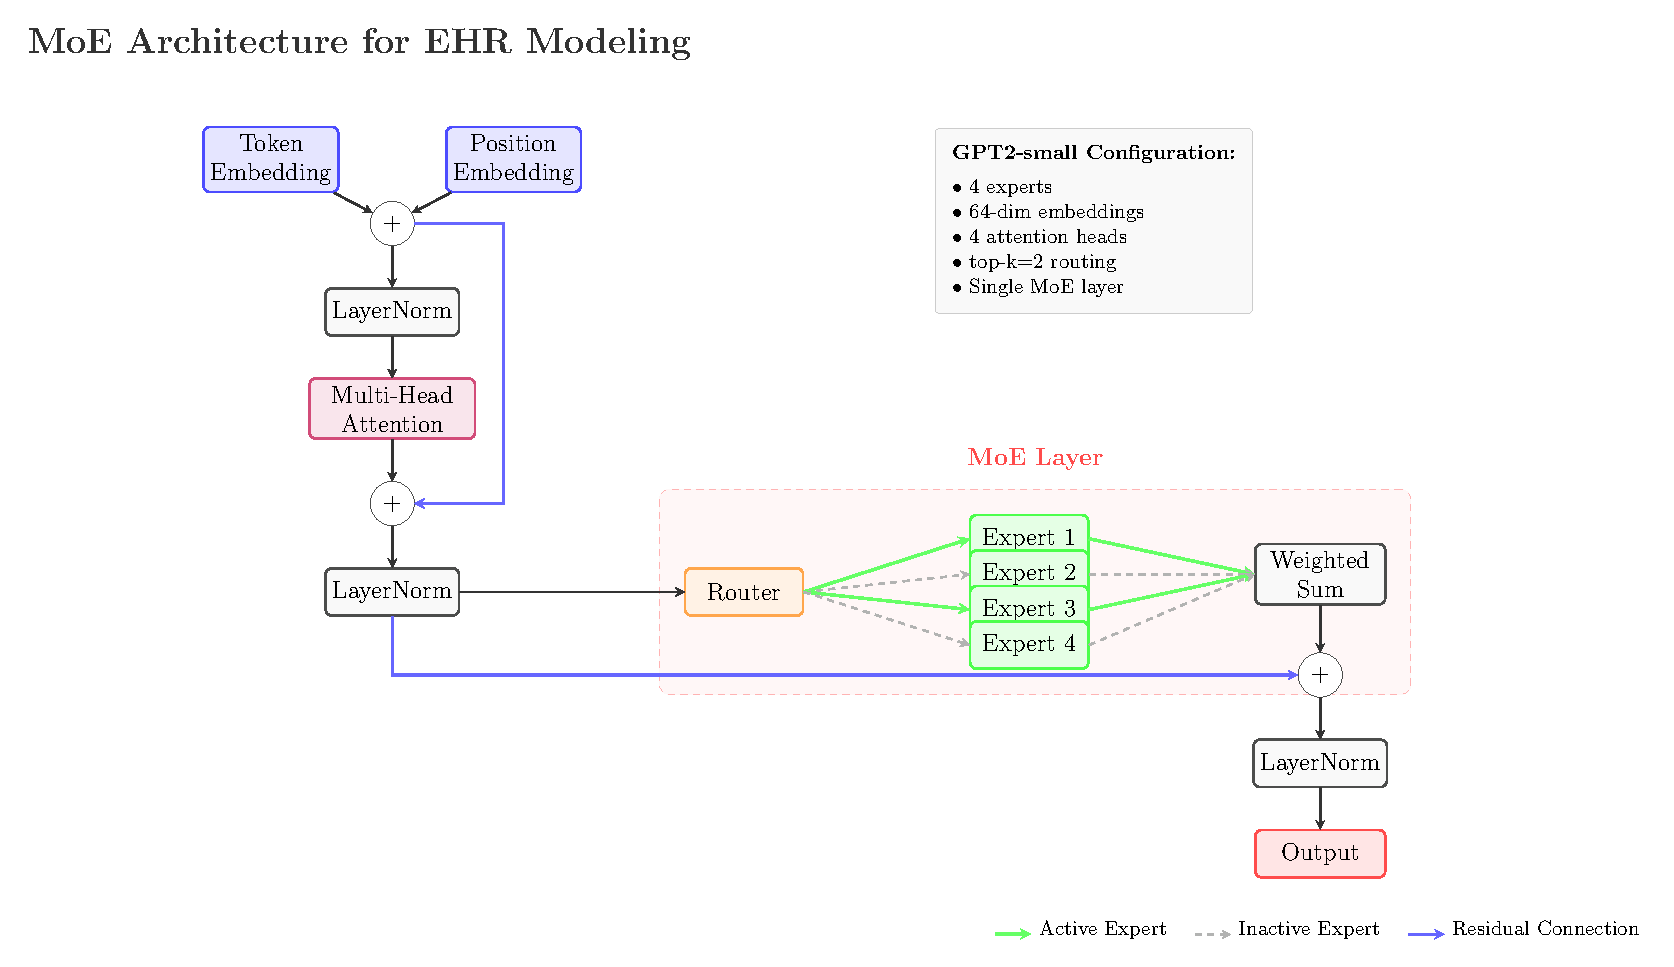
\includegraphics[width=1\colwidth]{figures/moe_architecture_horizontal.pdf}
          \caption{\large MoE Architecture for EHR Modeling}
          \label{fig:moe_architecture}
      \end{figure}

  \end{block}


  % \begin{block}{Machine Learning Interpretability}

  %   In machine learning, understanding how models make decisions is crucial. Interpretability reveals the reasoning behind predictions, while explainability provides insights into model behavior.
    

  %   \begin{figure}
  %     \centering
  %     \begin{tikzpicture}[scale=6]
  %       \draw[step=0.25cm,color=gray] (-1,-1) grid (1,1);
  %       \draw (1,0) -- (0.2,0.2) -- (0,1) -- (-0.2,0.2) -- (-1,0)
  %         -- (-0.2,-0.2) -- (0,-1) -- (0.2,-0.2) -- cycle;
  %     \end{tikzpicture}
  %     \caption{A figure caption.}
  %   \end{figure}

  %   Lorem ipsum dolor sit amet, consectetur adipiscing elit. Morbi ultricies
  %   eget libero ac ullamcorper. Integer et euismod ante. Aenean vestibulum
  %   lobortis augue, ut lobortis turpis rhoncus sed. Proin feugiat nibh a
  %   lacinia dignissim. Proin scelerisque, risus eget tempor fermentum, ex
  %   turpis condimentum urna, quis malesuada sapien arcu eu purus.

  % \end{block}

  % \begin{block}{A block containing a list}

  %   Nam vulputate nunc felis, non condimentum lacus porta ultrices. Nullam sed
  %   sagittis metus. Etiam consectetur gravida urna quis suscipit.

  %   \begin{itemize}
  %     \item \textbf{Mauris tempor} risus nulla, sed ornare
  %     \item \textbf{Libero tincidunt} a duis congue vitae
  %     \item \textbf{Dui ac pretium} morbi justo neque, ullamcorper
  %   \end{itemize}

  %   Eget augue porta, bibendum venenatis tortor.

  % \end{block}

  % \begin{alertblock}{A highlighted block}

  %   This block catches your eye, so \textbf{important stuff} should probably go
  %   here.

  %   Curabitur eu libero vehicula, cursus est fringilla, luctus est. Morbi
  %   consectetur mauris quam, at finibus elit auctor ac. Aliquam erat volutpat.
  %   Aenean at nisl ut ex ullamcorper eleifend et eu augue. Aenean quis velit
  %   tristique odio convallis ultrices a ac odio.

  %   \begin{itemize}
  %     \item \textbf{Fusce dapibus tellus} vel tellus semper finibus. In
  %       consequat, nibh sed mattis luctus, augue diam fermentum lectus.
  %     \item \textbf{In euismod erat metus} non ex. Vestibulum luctus augue in
  %       mi condimentum, at sollicitudin lorem viverra.
  %     \item \textbf{Suspendisse vulputate} mauris vel placerat consectetur.
  %       Mauris semper, purus ac hendrerit molestie, elit mi dignissim odio, in
  %       suscipit felis sapien vel ex.
  %   \end{itemize}

  %   Aenean tincidunt risus eros, at gravida lorem sagittis vel. Vestibulum ante
  %   ipsum primis in faucibus orci luctus et ultrices posuere cubilia Curae.

  % \end{alertblock}

  % \begin{block}{End-to-End Training Pipeline}

  %   \begin{enumerate}
  %       \item \textbf{Model Initialization:} GPT-2 backbone with MoE layers replacing standard MLPs
  %       \item \textbf{MoE Routing:} Top-k gating network selects relevant experts per token using learned router weights
  %       \item \textbf{Expert Processing:} Only activated experts process tokens, reducing computational overhead
  %       \item \textbf{Load Balancing:} Auxiliary loss ensures uniform expert utilization during training
  %       % \item \textbf{Mixed Precision:} FP16/BFloat16 autocast with gradient scaling for memory efficiency
  %       % \item \textbf{Gradient Accumulation:} Micro-batching across multiple steps before optimizer update
  %       % \item \textbf{Distributed Training:} DDP synchronization with gradient clipping for stability
  %       % \item \textbf{Learning Rate Scheduling:} Cosine decay with warmup for optimal convergence
  %       \item \textbf{Clinical Monitoring:} Special tokens for patient mortality, admission, and discharge are given more importance during training.
  %       % \item \textbf{Checkpointing:} Best model selection based on validation loss with comprehensive logging
  %   \end{enumerate}

  % \end{block}


  % \begin{alertblock}{Key Results}
    
  %   \textbf{Performance and Efficiency Improvements:}
  %   \begin{itemize}
  %       \item MoE model achieves state-of-the-art results in next-token prediction.
  %       \item The models scale much better by adding experts with minimal cost to inference.
  %       \item Matches monolithic model accuracy on downstream tasks.
  %       \item Sparse activation reduces GPU memory usage during inference
  %       \item Experts learn distinct clinical concepts, improving interpretability.
  %       \item Pruning experts for specific tasks boosts speed and saves memory.
  %       \item Converges faster with significantly less computational cost (FLOPs).
  %   \end{itemize}
    
  %   \textbf{Clinical Deployment Benefits:}
  %   \begin{itemize}
  %       \item Suitable for resource-constrained clinical settings
  %       \item Real-time inference capabilities
  %       \item Reduced infrastructure requirements
  %       \item Cost-effective scaling for hospital systems
  %   \end{itemize}

  % \end{alertblock}






  \begin{block}{Experimental Results}
    
    \begin{figure}
      \centering
      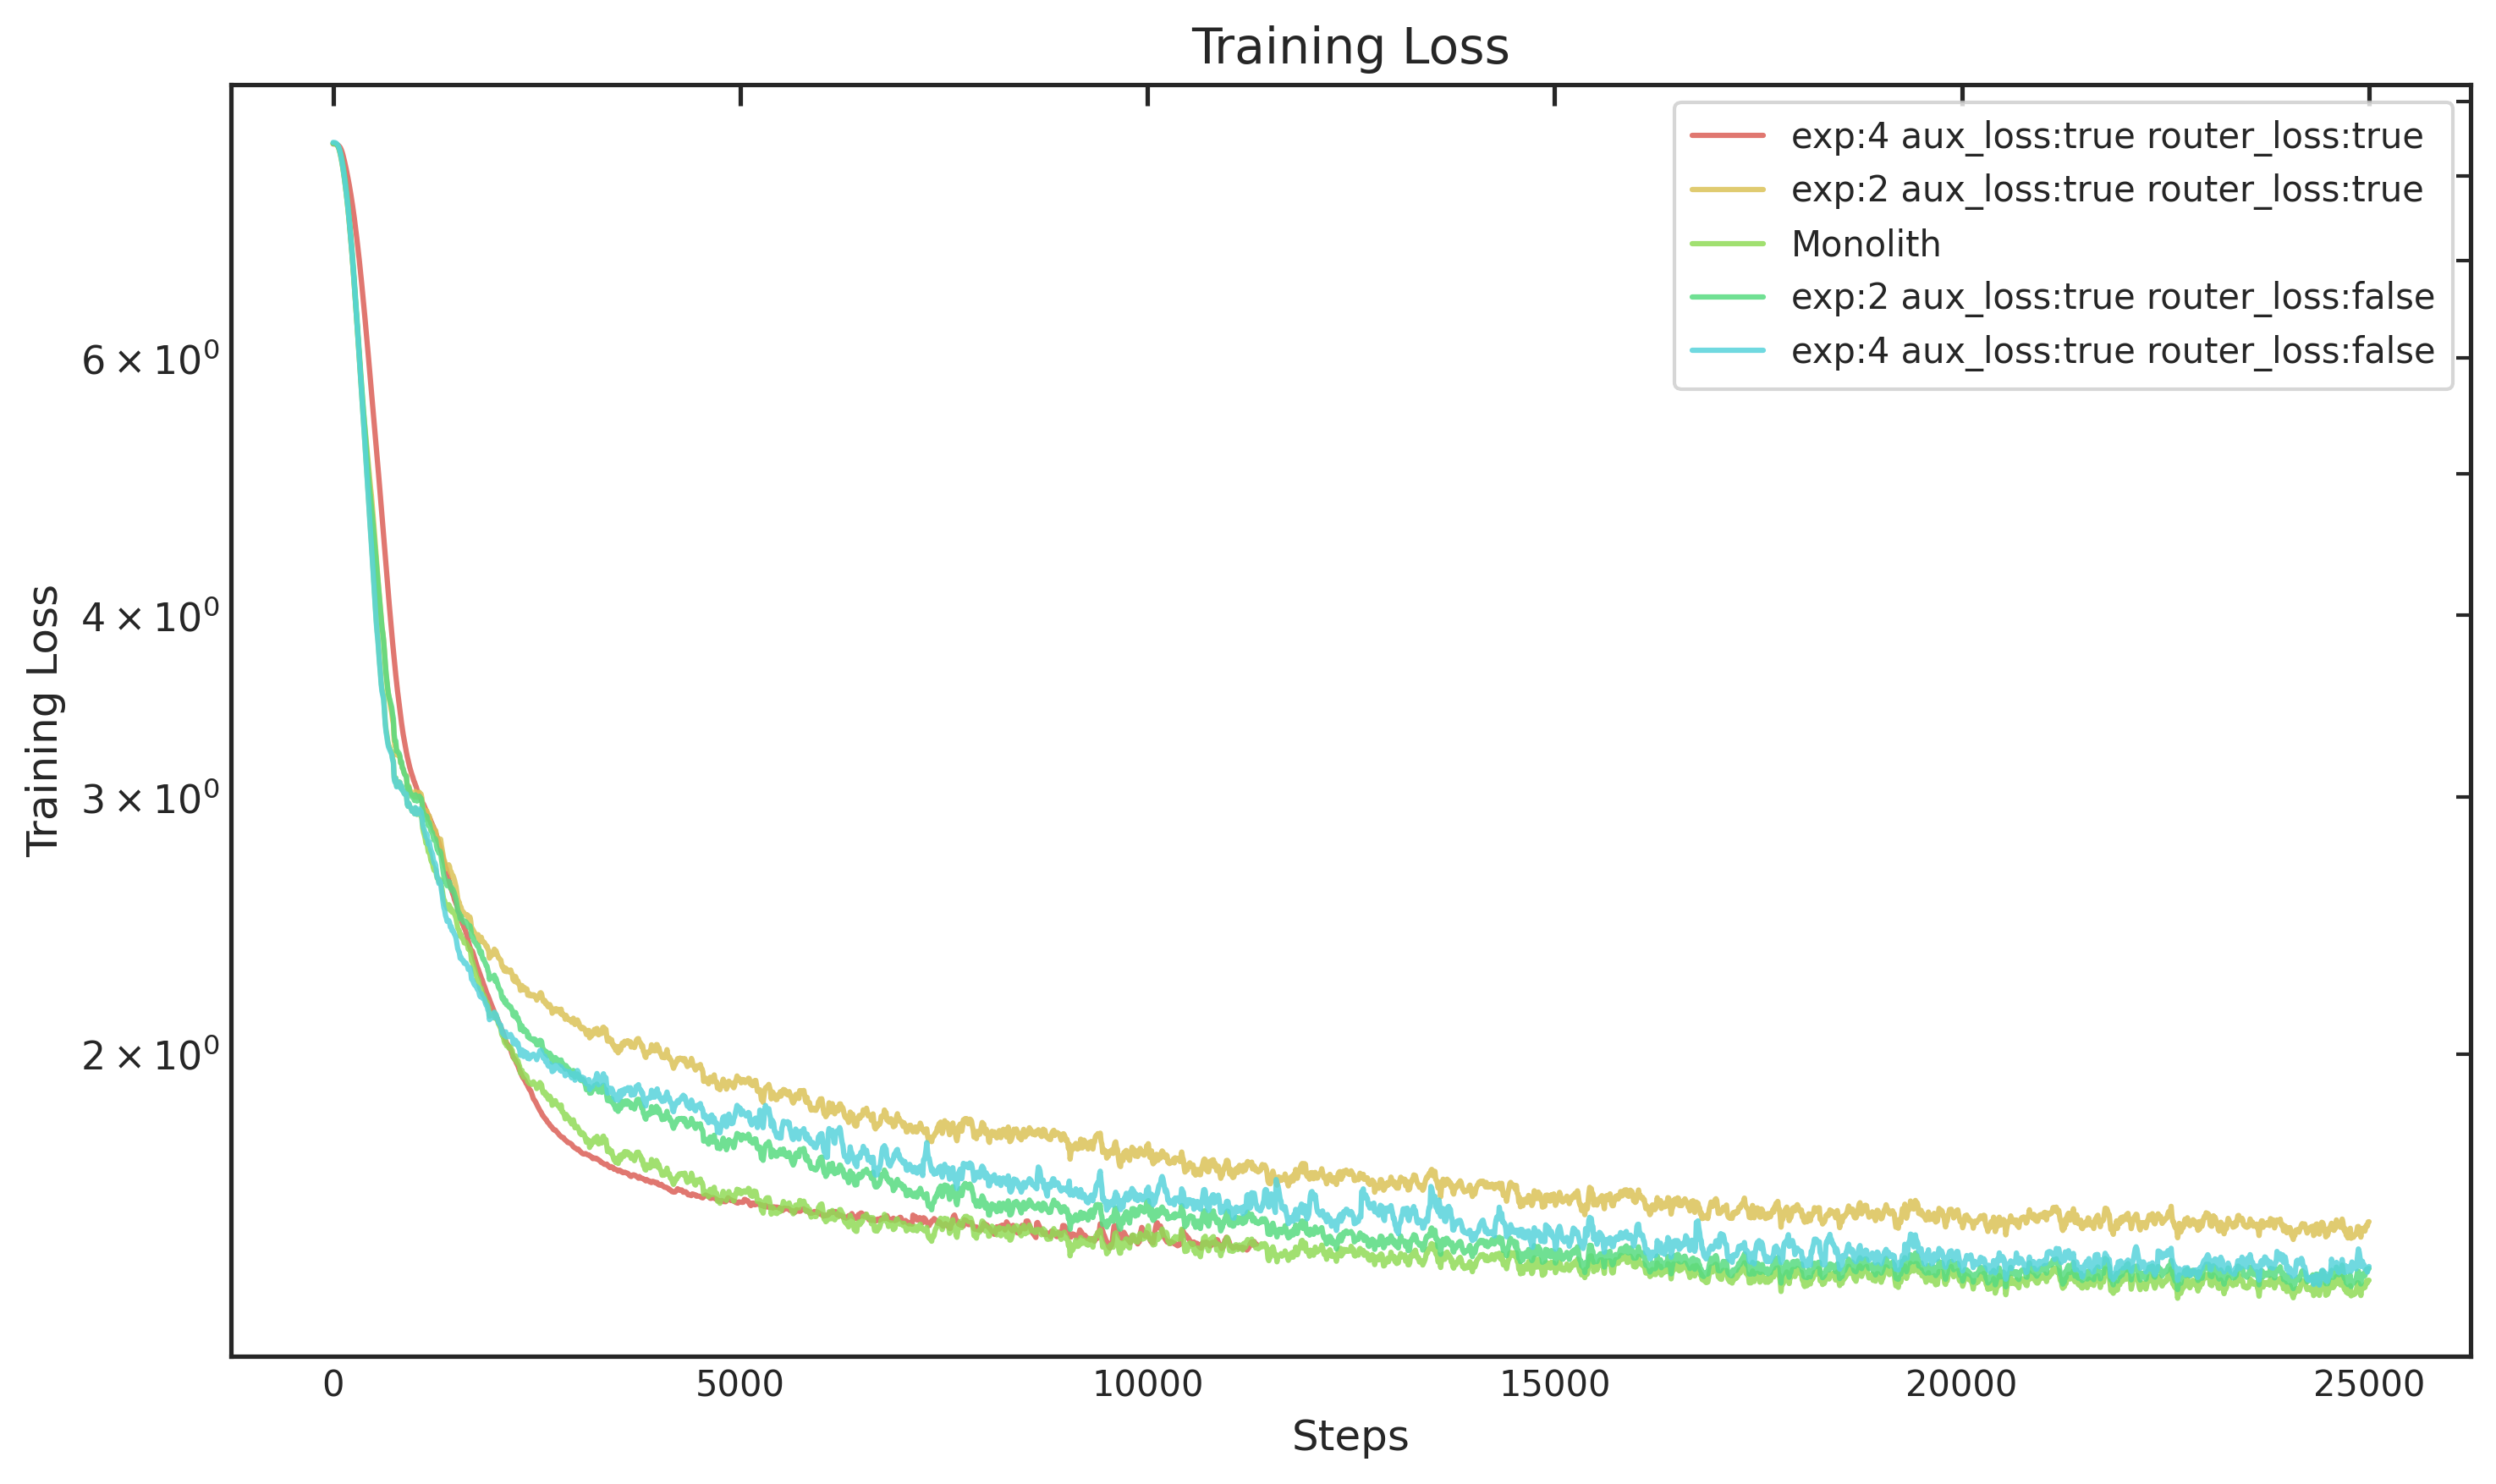
\includegraphics[width=1\linewidth]{figures/loss_curve.png}
      % \caption{Loss Curves: MoE vs Dense Models}
      \label{fig:loss_curve}
   \end{figure}

    \textbf{Evaluation Metrics:}
    \begin{itemize}
        \item \textbf{Clinical Performance:} ROC-AUC, accuracy, precision, and recall for clinical NTP tasks
        \item \textbf{Model Efficiency:} Parameter count comparison and computational complexity analysis (MACs and FLOPs operations)
        \item \textbf{Training Dynamics:} Convergence rate, training time, and resource utilization metrics
        \item \textbf{Inference Performance:} Batch processing latency, throughput, and memory consumption during validation
    \end{itemize}
    
    \footnotesize
    \begin{table}[htbp]
    \centering
    % \caption{Experiment Results Comparison}
    \begin{tabular}{|l|c|c|c|c|c|}
    \hline
    \textbf{Configuration} & \textbf{Monolith} & \textbf{n\_exp=4, aux=T, z\_loss=F} & \textbf{n\_exp=2, aux=T, z\_loss=F} & \textbf{n\_exp=4, aux=T, z\_loss=T} & \textbf{n\_exp=2, aux=T, z\_loss=T} \\
    % \textbf{Experiment ID} & \textbf{2025-05-14/02-53-17} & \textbf{2025-05-14/07-48-34} & \textbf{2025-05-14/07-39-46} & \textbf{2025-05-14/00-56-55} & \textbf{2025-05-12/13-38-13} \\
    \hline
    \hline
    \multicolumn{6}{|c|}{\textbf{All Tokens (Top-3)}} \\
    \hline
    Accuracy & \textbf{0.759} & \textcolor{red}{0.752} & \textcolor{blue}{0.746} & 0.735 & 0.721 \\
    Precision & \textbf{0.253} & \textcolor{red}{0.251} & \textcolor{blue}{0.249} & 0.245 & 0.240 \\
    Recall & \textbf{0.759} & \textcolor{red}{0.752} & \textcolor{blue}{0.746} & 0.735 & 0.721 \\
    \hline
    \hline
    \multicolumn{6}{|c|}{\textbf{MEDS\_DEATH}} \\
    \hline
    ROC-AUC & \textbf{0.997} & \textcolor{red}{0.995} & \textcolor{blue}{0.994} & 0.993 & 0.991 \\
    Accuracy (Top-3) & \textcolor{red}{0.050} & \textcolor{blue}{0.033} & \textcolor{blue}{0.033} & \textbf{0.139} & \textcolor{blue}{0.033} \\
    Precision (Top-3) & \textbf{0.273} & \textcolor{blue}{0.091} & \textcolor{blue}{0.091} & \textcolor{red}{0.155} & 0.030 \\
    Recall (Top-3) & \textcolor{red}{0.182} & \textcolor{blue}{0.091} & \textcolor{blue}{0.091} & \textbf{0.241} & \textcolor{blue}{0.091} \\
    \hline
    \hline
    \multicolumn{6}{|c|}{\textbf{HOSPITAL\_ADMISSION}} \\
    \hline
    ROC-AUC & \textcolor{red}{0.998} & \textcolor{red}{0.998} & \textbf{0.999} & \textcolor{red}{0.998} & \textcolor{red}{0.998} \\
    Accuracy (Top-3) & \textbf{0.859} & 0.807 & \textcolor{red}{0.839} & 0.758 & \textcolor{blue}{0.843} \\
    Precision (Top-3) & \textcolor{red}{0.379} & \textcolor{blue}{0.339} & \textbf{0.388} & 0.349 & 0.251 \\
    Recall (Top-3) & \textcolor{red}{0.833} & \textbf{0.834} & \textcolor{blue}{0.827} & 0.776 & 0.801\\
    \hline
    \hline
    \multicolumn{6}{|c|}{\textbf{HOSPITAL\_DISCHARGE}} \\
    \hline
    ROC-AUC & \textbf{0.996} & \textcolor{blue}{0.995} & \textbf{0.996} & \textcolor{blue}{0.995} & \textcolor{blue}{0.995} \\
    Accuracy (Top-3) & \textcolor{red}{0.590} & 0.559 & \textbf{0.640} & \textcolor{blue}{0.578} & 0.546 \\
    Precision (Top-3) & \textbf{0.301} & \textcolor{red}{0.282} & \textcolor{blue}{0.258} & 0.250 & 0.241 \\
    Recall (Top-3) & \textcolor{red}{0.622} & \textcolor{blue}{0.591} & \textbf{0.671} & 0.585 & 0.552 \\
    \hline
    \end{tabular}
    \end{table}
    
 
    
  \end{block}

  % \begin{block}{Conclusions \& Future Work}
    
  %   \textbf{Contributions:}
  %   \begin{itemize}
  %       \item Novel MoE architecture for EHR foundational models
  %       \item Demonstrated efficiency gains without accuracy loss
  %       \item Validated on MIMIC-IV dataset with clinical tasks
  %   \end{itemize}

  %   \textbf{Future Directions:}
  %   \begin{itemize}
  %       \item Multi-modal integration (clinical notes, imaging)
  %       \item Federated learning for multi-hospital deployment
  %       \item Expert interpretability and clinical validation
  %       \item Real-world clinical trial implementation
  %   \end{itemize}
    
  % \end{block}
        
\end{column}

\separatorcolumn
\end{columns}
\end{frame}

\end{document}
